\documentclass[letter,12pt]{article}

\usepackage{amsmath}
\usepackage{amssymb}
\usepackage{graphicx,psfrag}
\usepackage{geometry}
\usepackage{subfigure}
\usepackage{url}
\geometry{left=3cm, right=3cm, top=2cm,bottom=4 cm}
\usepackage{hyperref}
\hypersetup{colorlinks=true}
% define the title
\author{Armin Eftekhari, Alejandro Weinstein}
\title{ Data Mining, Project 5 report\\
Mining Flickr}
\date{December 4, 2009}

\setlength{\parindent}{0in}
%\setlength{\mathindent}{0in}
\addtolength{\parskip}{5pt}

\def\etal{\mbox{\textit{et al. }}}
\newcommand{\vect}[1]{\boldsymbol{#1}}

\begin{document}
\maketitle

\section{Introduction}

Flickr is one of the most popular image hosting website, with more than 4 billion pictures \cite{wiki_flickr}. For each picture, the community can add comments, tags, or call the picture his or her favorite. Also, the details of the camera used to take the picture are available. So, an interesting question arise: is there any correlation between the popularity of a photo and the camera used to take it? The purpose of this project is to try to answer this, and to find other interesting patterns.

\section{Generating the data set}

There is no dataset directly available with the data needed to analyze Flickr. However, there is a Flickr API that allows to build such dataset. We wrote a Python script, using the Python ``Flickr API kit'' \cite{ web_flickr_api} to do that.

We decided to build a dataset with the following attributes:
\begin{description}
\item[Id:] the unique id used by Flickr to identify a photo.
\item[Views:] the number of views of the photo.
\item[Location:] the location of the photo.
\item[Comments:] the number of comments of the photo.
\item[Tags:] the number of tags of the photo.
\item[Favorites:] the number of Flickr users that call the photo a favorite.
\item[Make:] the maker of the camera used to take the photo.
\item[Model:] the model of the camera used to take the photo.
\end{description}

Since it is not feasible to get information about all the pictures in Flickr, a key point at the moment of building the dataset is to determine how to sample the website. We decided to get the data of 100 picture for each of the most popular tags. Unfortunately, we didn't find an API function to get the most popular tags, so we copy the list of the most popular tags from the ``All time most popular tags'' page \cite{web_flickr_tags}. We also looked at photos at least one year old, to guarantee that the pictures has been exposed to the community for a time long enough.

We built the dataset in four steps:

\begin{enumerate}
\item Get the 100 ids for each of the popular tags: For each of the popular tags, we get the ids of 100 photos. In this step we ask for pictures at least one year old. We got 14400 records.
\item Eliminate the duplicate ids. Since a given photo can be associated to more than one tag, it is possible to have duplicated ids. We eliminated the duplicate ids, reducing the 14400 records to 7342.
\item Get the data for each photo id.
\item Write the data as a CSV file.
\end{enumerate}

It is interesting to note that the time Flickr take to respond to each API call is roughly one second, and consequently, building the dataset took several hours.

The examination of the dataset revealed that the \emph{Make} attribute was inconsistent, since we got slightly different names for a given maker. For instance, ``Olympus'' cameras were labeled as ``Olympus Imaging Corp.'', ``Olympus optical Co. Ltd'' or ``Olympus corporation''. We wrote another Python script to solve this inconsistency, reducing the number of unique manufacturers from 62 to 36.

\section{Summary statistics}

After finishing the preprocessing of the dataset, the next step on the data mining process is to generate some summary statistics, to get a general idea of the structure of the data. Table \ref{tbl:stat_num} shows the statistics for the numerical attributes. For the categorical attributes ``make'' and ``model'', the mode is ``Canon'' and ``Nikon D200'', respectively.

\begin{table}[!h]
%\caption{Statistics for the ``views'' attribute}
\centering
\caption{Summary statistics for the numerical attributes.}
\label{tbl:stat_num}
\subtable{
\begin{tabular}{|l|l|}
\hline\multicolumn{2}{|c|}{views} \\
\hline
Min & 164 \\
Max & 1184897 \\
Mean & 14778.5\\
Std dev & 35718.6 \\
\hline
\end{tabular}}
\subtable{
\begin{tabular}{|l|l|}
\hline\multicolumn{2}{|c|}{comments} \\
\hline
Min & 6 \\
Max & 2891 \\
Mean & 150.2\\
Std dev & 161.8 \\
\hline
\end{tabular}}
\subtable{
\begin{tabular}{|l|l|}
\hline\multicolumn{2}{|c|}{tags} \\
\hline
Min & 2 \\
Max & 279 \\
Mean & 30.2\\
Std dev & 17.5 \\
\hline
\end{tabular}}
\subtable{
\begin{tabular}{|l|l|}
\hline\multicolumn{2}{|c|}{favorites} \\
\hline
Min & 0 \\
Max & 8539 \\
Mean & 243.0\\
Std dev & 348.2 \\
\hline
\end{tabular}}
\end{table}

Figure \ref{fig:histo_numerical} shows the histograms for the numerical attributes. As can be seen, all the numerical attributes share a \emph{long tail} behavior, where most of the photos are unpopular (in terms of a low number of views, comments, etc), and a relatively small amount of the photos are very popular. Figure \ref{fig:histo_make} shows an histogram for the ``Make'' attribute. First of all, it can be noted that a significant amount of the photos (44\%) don't have information about the maker of the camera used to take the picture. As we will discuss later in section \ref{sec:classifier}, this will play a detrimental role in our data mining analysis. Secondly, we can see that the two mayor players are \emph{Canon} and \emph{Nikon}, followed by a handful of other brands with a significant share of the photos. Most of the remaining manufactures are associated with only one photo.

\begin{figure}[!h]
\centering
\subfigure[``Views'' histogram]{
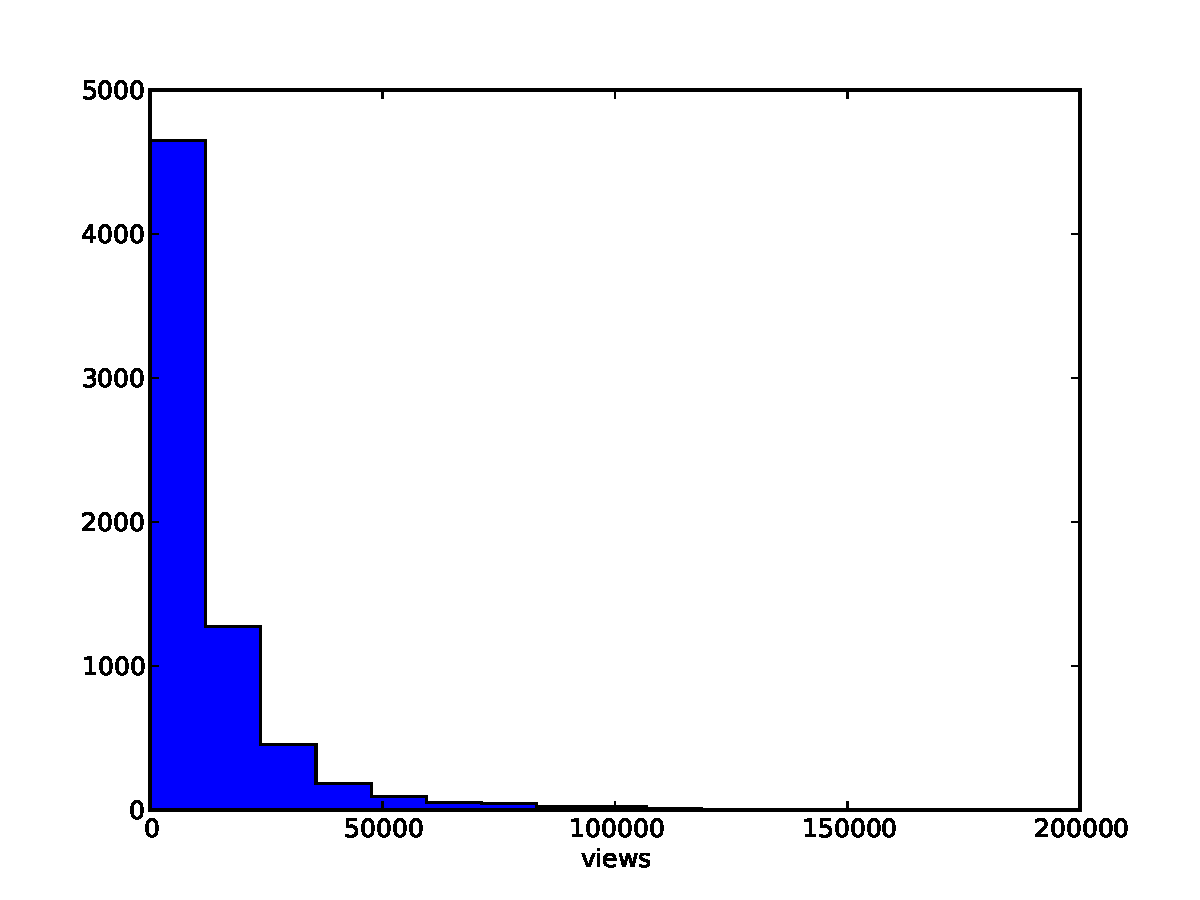
\includegraphics[scale=0.35]{histo_views.pdf}
}
\subfigure[``Comments'' histogram]{
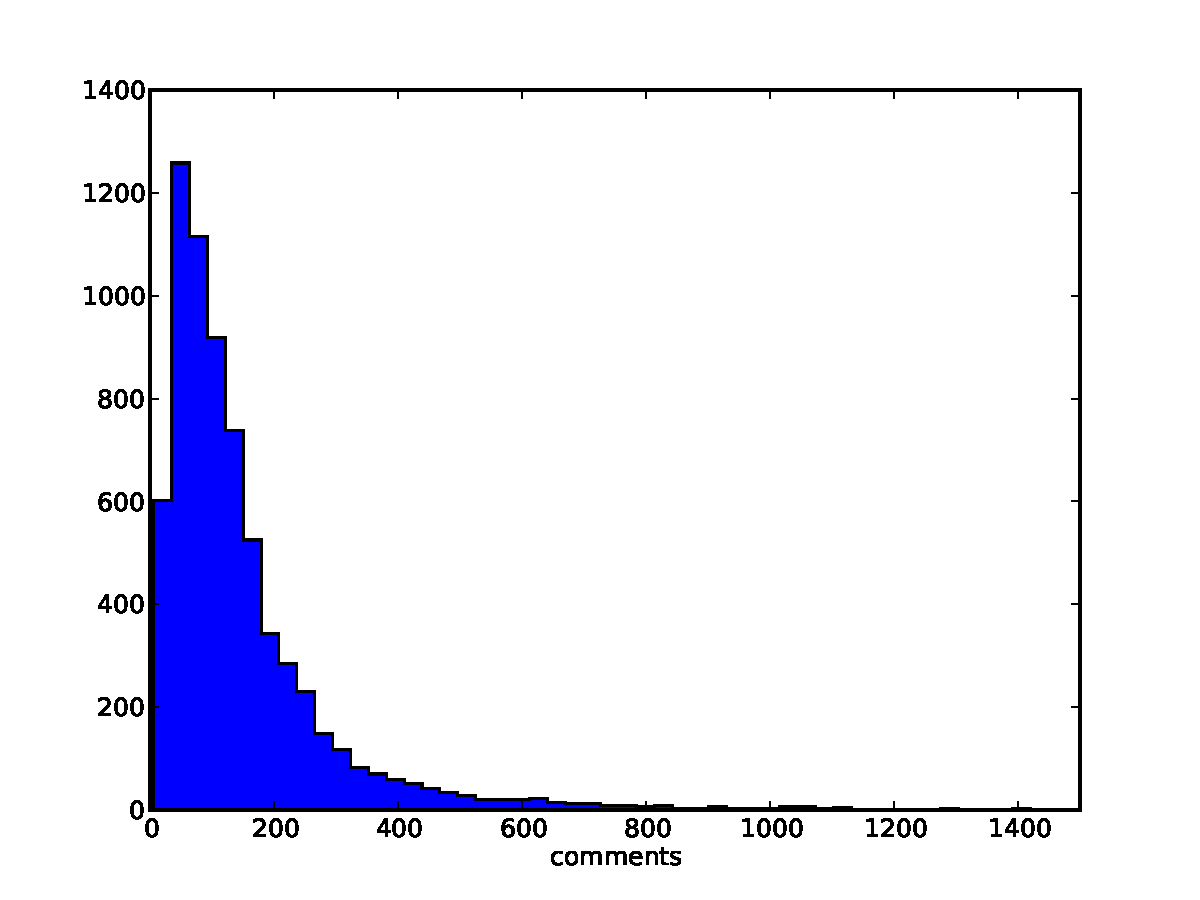
\includegraphics[scale=0.35]{histo_comments.pdf}
}
\subfigure[``Tags'' histogram]{
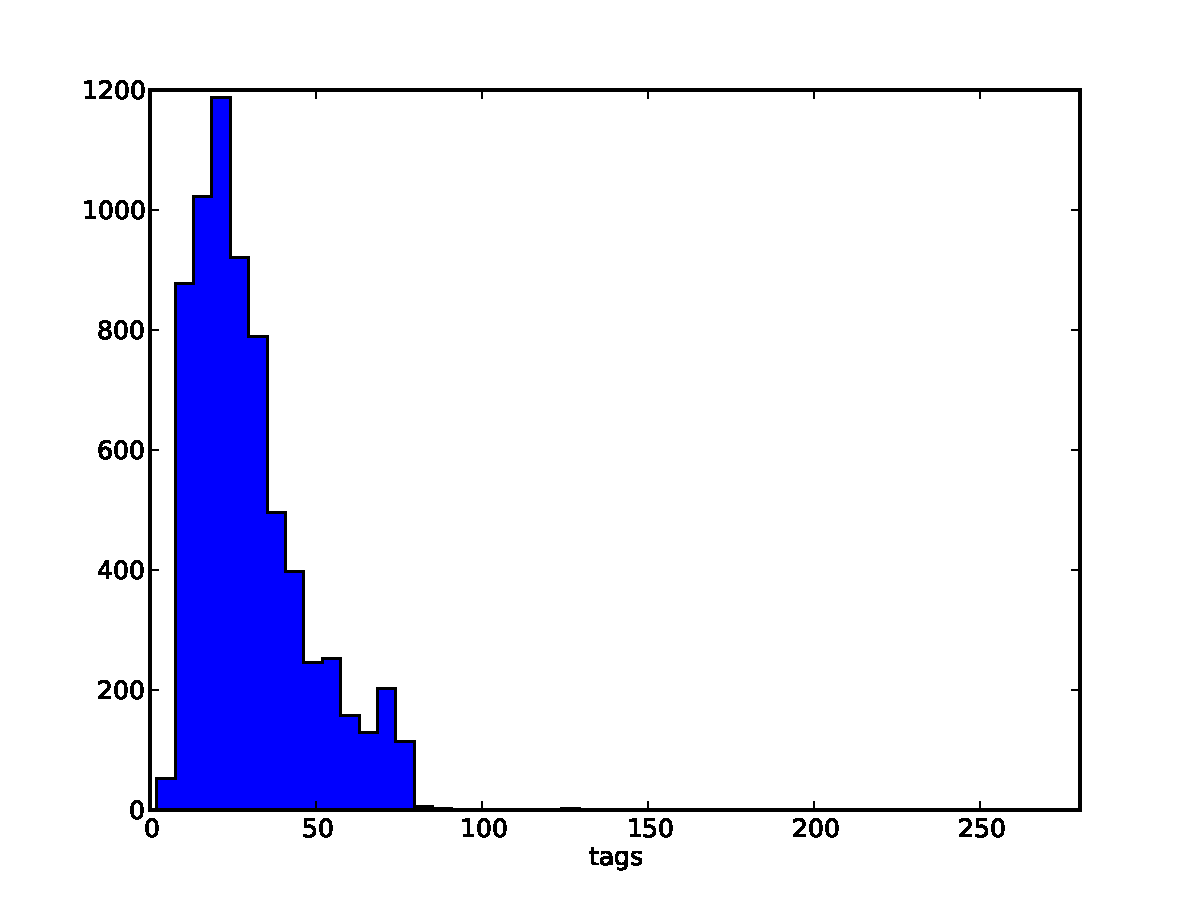
\includegraphics[scale=0.35]{histo_tags.pdf}
}
\subfigure[``Favorites'' histogram]{
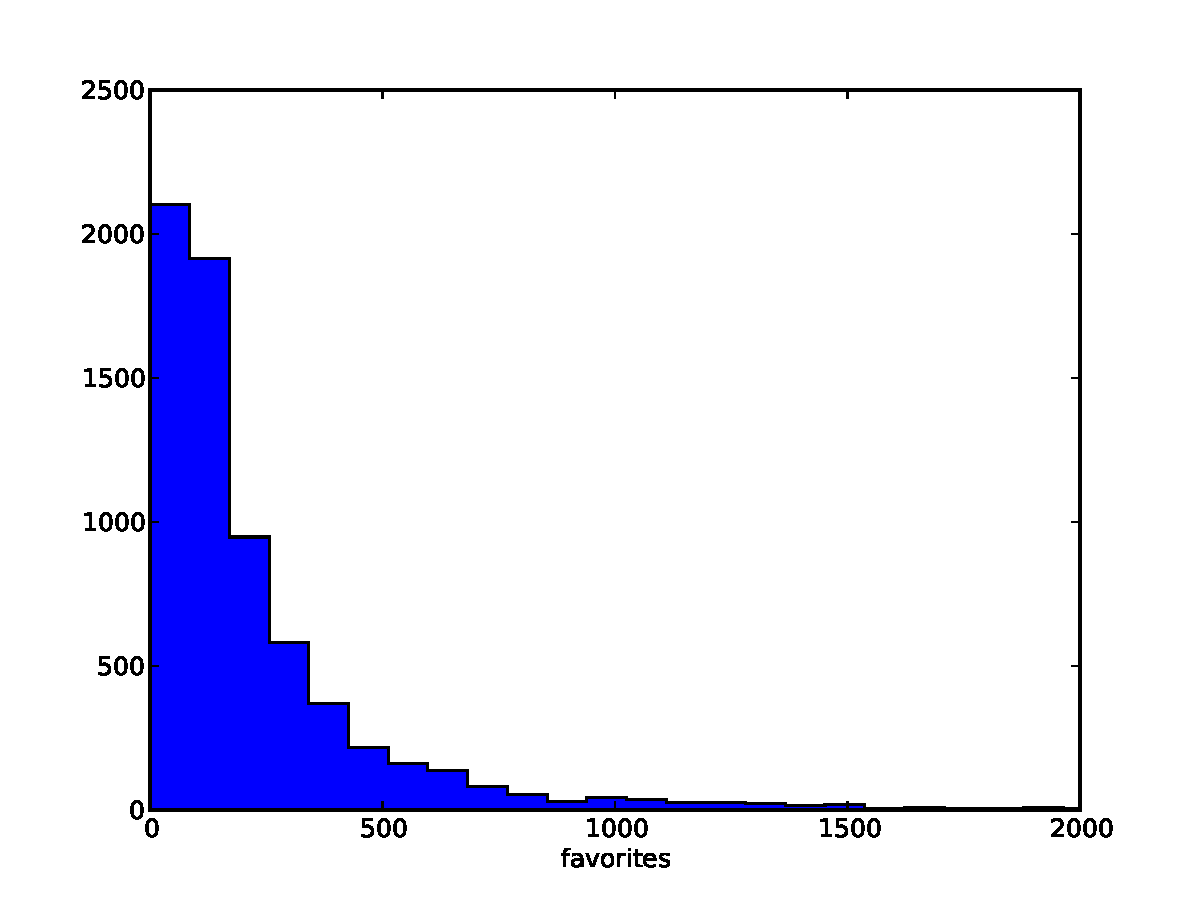
\includegraphics[scale=0.35]{histo_favorites.pdf}
}
\caption{Histogram for ``views'', ``comments'', ``tags'' and ``favorites''.}
\label{fig:histo_numerical}
\end{figure}

\begin{figure}[!h]
\centering
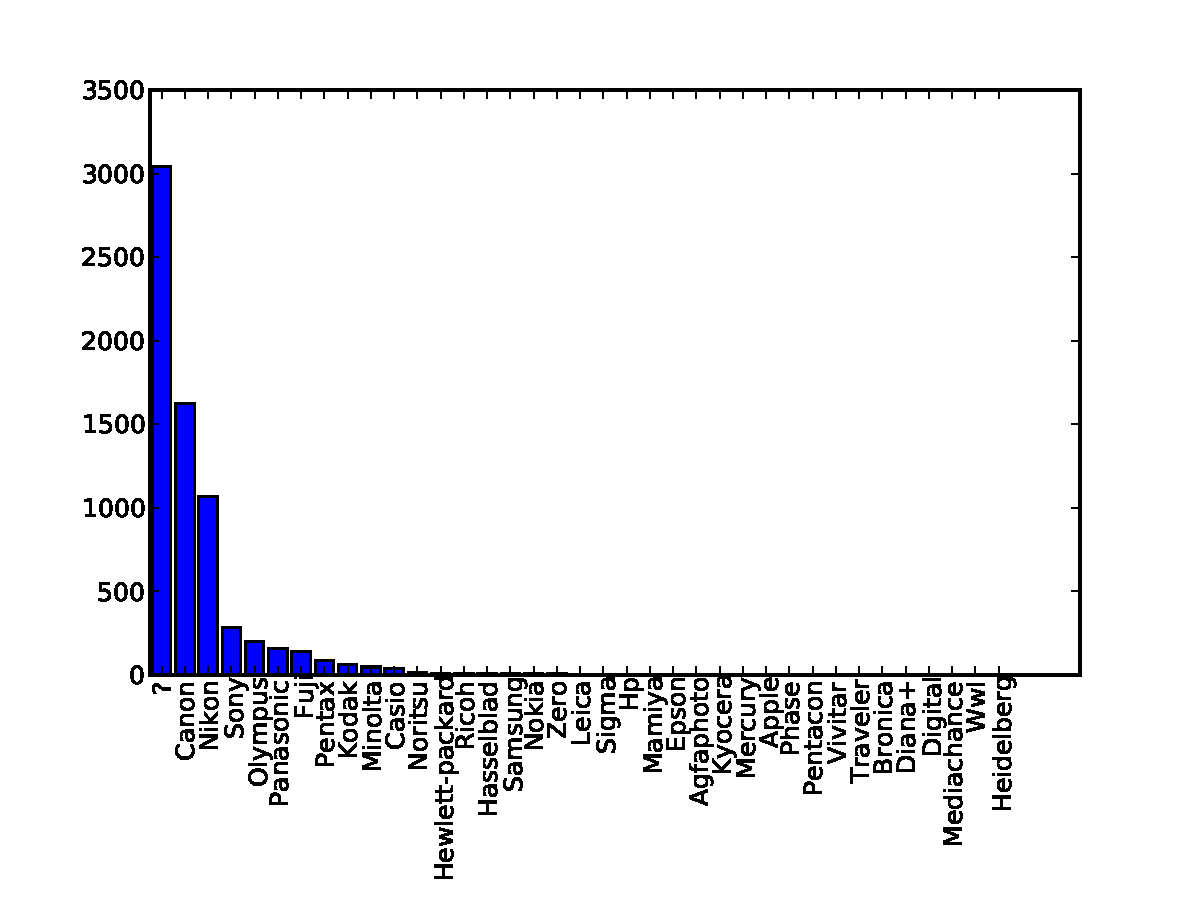
\includegraphics[scale=0.6]{histo_make.pdf}
\caption{Histogram for the ``maker'' attribute.}
\label{fig:histo_make}
\end{figure}

Figure \ref{fig:scatter} shows a scatter plot, where the $x$ axis correspond to the number of comments and the $y$ axis correspond to the number of views. The color of each point is mapped to the logarithm of the number of favorites\footnote{A logarithmic map is used due to the huge range of the variable. Otherwise, most of the points end with the same color}. This plot illustrate, once again, the \emph{long tail} behavior of the data, where we can see a big cluster of photos close to the origin, and a set of very popular outliers.

Notice that all the plots for the summary statistics were produced using Python and the Matplotlib library, since we think that the ones produced by Weka are very low quality.

\begin{figure}[!h]
\centering
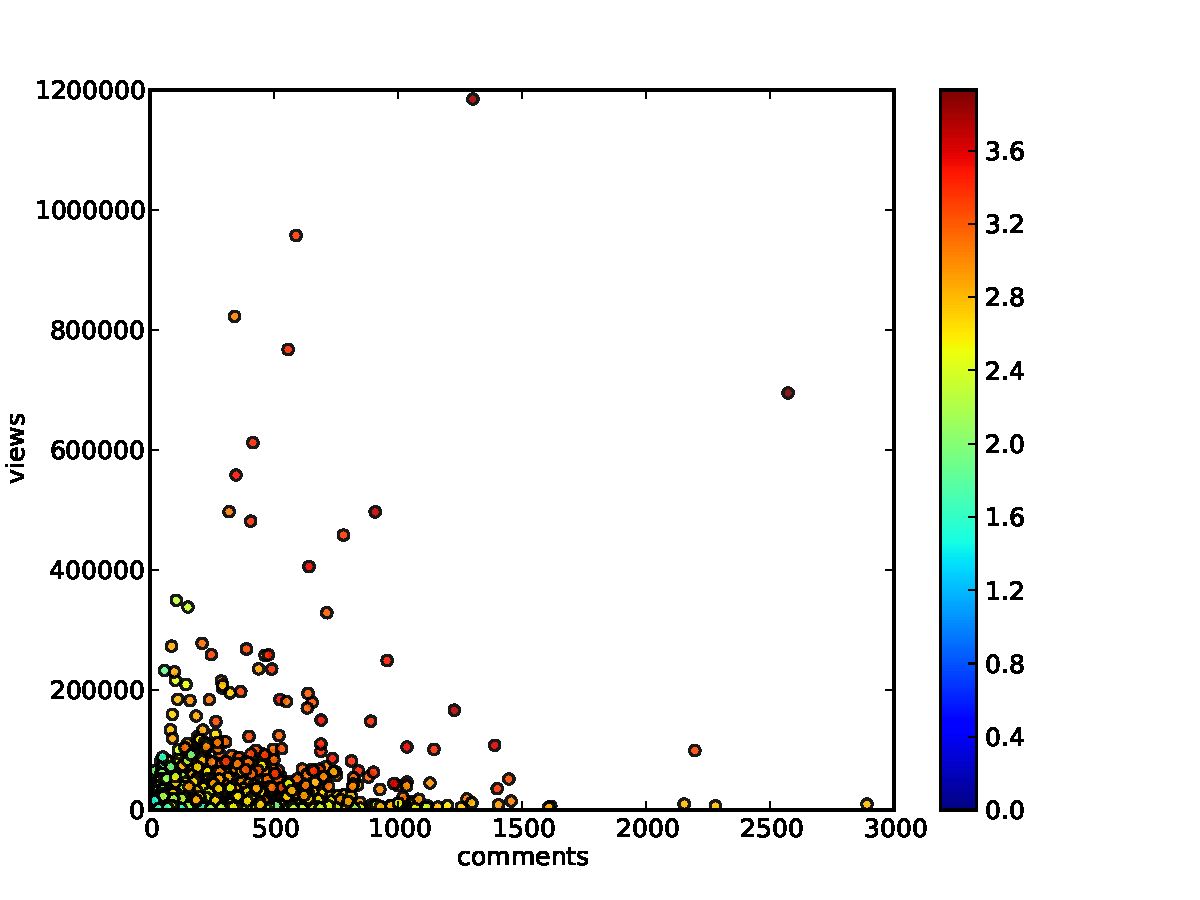
\includegraphics[scale=0.6]{scatter.pdf}
\caption{Scatter plot. The color represent the logarithmic of the ``favorite'' attribute.}
\label{fig:scatter}
\end{figure}

\section{Clustering}

\subsection{Location}

Here we were interested in the location of Flickr users. In particular,
we wanted to study any possible relations between the clusters and
the location of users. Typically, social networks are more likely
to form among people who live nearby, have the same language, and share
the same culture. So, we expected to observe a distinct relation between
the clusters and the location of Flickr users. First, user ID was
omitted from our attributes. Then typical k-means clustering was performed
on data using 100 iterations. You can observe the cluster centers
below.

%
\begin{table}
\centering
\begin{tabular}{|c|c|c|}
\hline
Cluster No. & Number of records & Location\tabularnewline
\hline
\hline
1 & 532 & San Francisco USA\tabularnewline
\hline
2 & 440 & San Francisco USA\tabularnewline
\hline
3 & 726 & Livermore \& Antioch Calif. USA\tabularnewline
\hline
4 & 817 & New York U.S.A.\tabularnewline
\hline
5 & 1352 & San Francisco USA \tabularnewline
\hline
6 & 478 & Bonn Germany\tabularnewline
\hline
7 & 278 & the Island of Mactan Cebu Philippines\tabularnewline
\hline
8 & 265 & Berlin Germany\tabularnewline
\hline
9 & 1507 & Tokyo Japan \tabularnewline
\hline
10 & 571 & Barcelona Spain\tabularnewline
\hline
\end{tabular}
\caption{Relation between cluster centroid and locations}
\end{table}

We first see that all the locations are basically tourist destinations
and that, as stated above, they belong to different clusters and different
social networks. Interestingly these results also tell us that San
Francisco in U.S. and Tokyo in Japan are very popular tourist destinations
among others.

\subsection{Comments}

Even before this analysis, we expected a close relation between number
of comments on a image and the number of people who marked that image
as favorite. After clustering, it turned out that there is a semi-linear
relation between them, as observed in Figure \ref{Flo:comm_fav}.
However, this relation doesn't remain exactly linear and there are
many images with many comments and yet few favorite marks, which is
interesting in its own right.


\begin{figure}
\centering
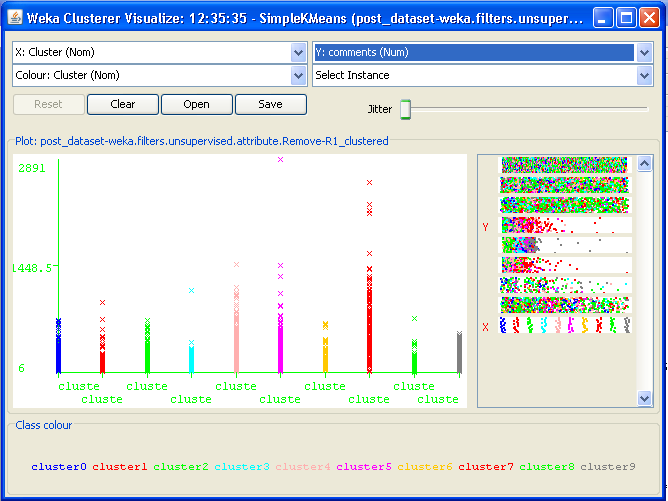
\includegraphics[width=0.8\textwidth]{clusno_comm.png}
\caption{Relation between the comments on an image and favorite status}
\label{Flo:comm_fav}
\end{figure}


Also it is instructive to study number of comments in each cluster,
which is summarized in Figure \ref{Flo:clus_comm}. Going to information
on the cluster centroid we find out that cluster 8 which has the
highest number of comments in average corresponds to Tokyo Japan.
Also, before running this analysis, we expected that photos which
are more viewed are likely to get more comments. Interestingly, it
turned out that there is not a clear and special relation between
these two, as one may see in Figure \ref{Flo:com_view}


\begin{figure}
\centering
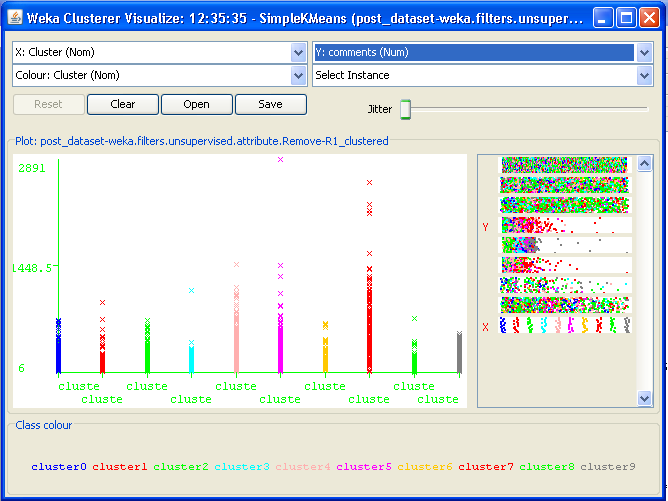
\includegraphics[width=0.8\textwidth]{clusno_comm.png}
\caption{Number of comments represented by each cluster}
\label{Flo:clus_comm}
\end{figure}


\begin{figure}
\centering
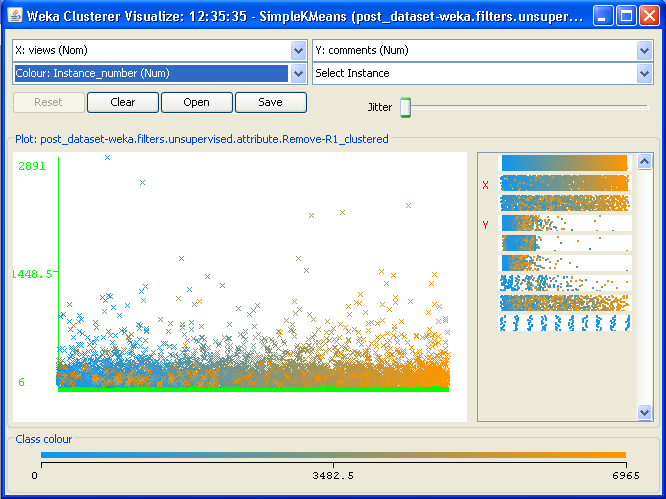
\includegraphics[width=0.8\textwidth]{comm_vew.png}
\caption{Relation between views and number of comments}
\label{Flo:com_view}
\end{figure}


\subsection{Camera Model}

Before we started the analysis, we hoped to find a relation between
the camera model and the favorite status of a photo. In practice,
however, we faced an unbalanced data which contained large number
of photos from fairly few camera models, such as Nikon D200. As a
result, patterns were not meaningful. In particular, let us show how
model and favorite status are related using the k-means clustering
(Figure \ref{Flo:model_fav}). This figure shows that there is clusters
with higher number of favorite images within, simply correspond to
Nikon D200 and then Canon EOS 5D, which is not meaningful, because
these are simply the most frequent camera models in dataset.


\begin{figure}
\centering
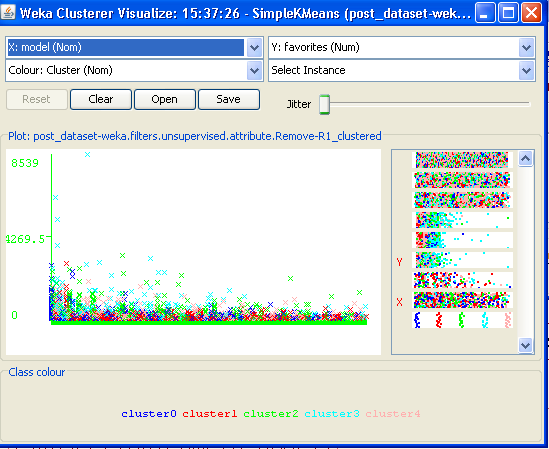
\includegraphics[width=0.8\textwidth]{fav_model.png}
\caption{Relation between camera model and favorite status}
\label{Flo:model_fav}
\end{figure}

\subsection{Other Clustering Algorithms}

In our analysis, we have used simple k-means clustering algorithm.
The main reason has been the efficiency and robustness of this clustering
technique. In particular, we tried several other clustering techniques
but the main problem was excessive computational requirements. In
contrast, k-means gives good results and is very fast and efficient.


\section{Classifiers}

\label{sec:classifier}

In this section we try to study the effect of different attributes
and the level of information that they carry. One of the ideas suggested
during our presentation was to design a classifier that predicts the
camera model. In fact, due to large imbalance in prior probabilities,
we can simply use the zero-R classifier and yet get pretty good classification
result. This is due to the fact that most of the photos in the dataset
are taken by few camera models.

So, we turn into another interesting problem, which studies the role
of camera model on the status of photo. In particular, due to mentioned
imbalance, we have to employ a classification technique that is least
sensitive to prior probabilities. One candidate is support vector
machines, because in SVM the classification boundary only depends
on support vectors and not on the prior probabilities. This is best
visualized in Figure \ref{Flo:SVM_balance}. Note that only a very
few number samples actually contribute to the boundary.

%
\begin{figure}
\centering
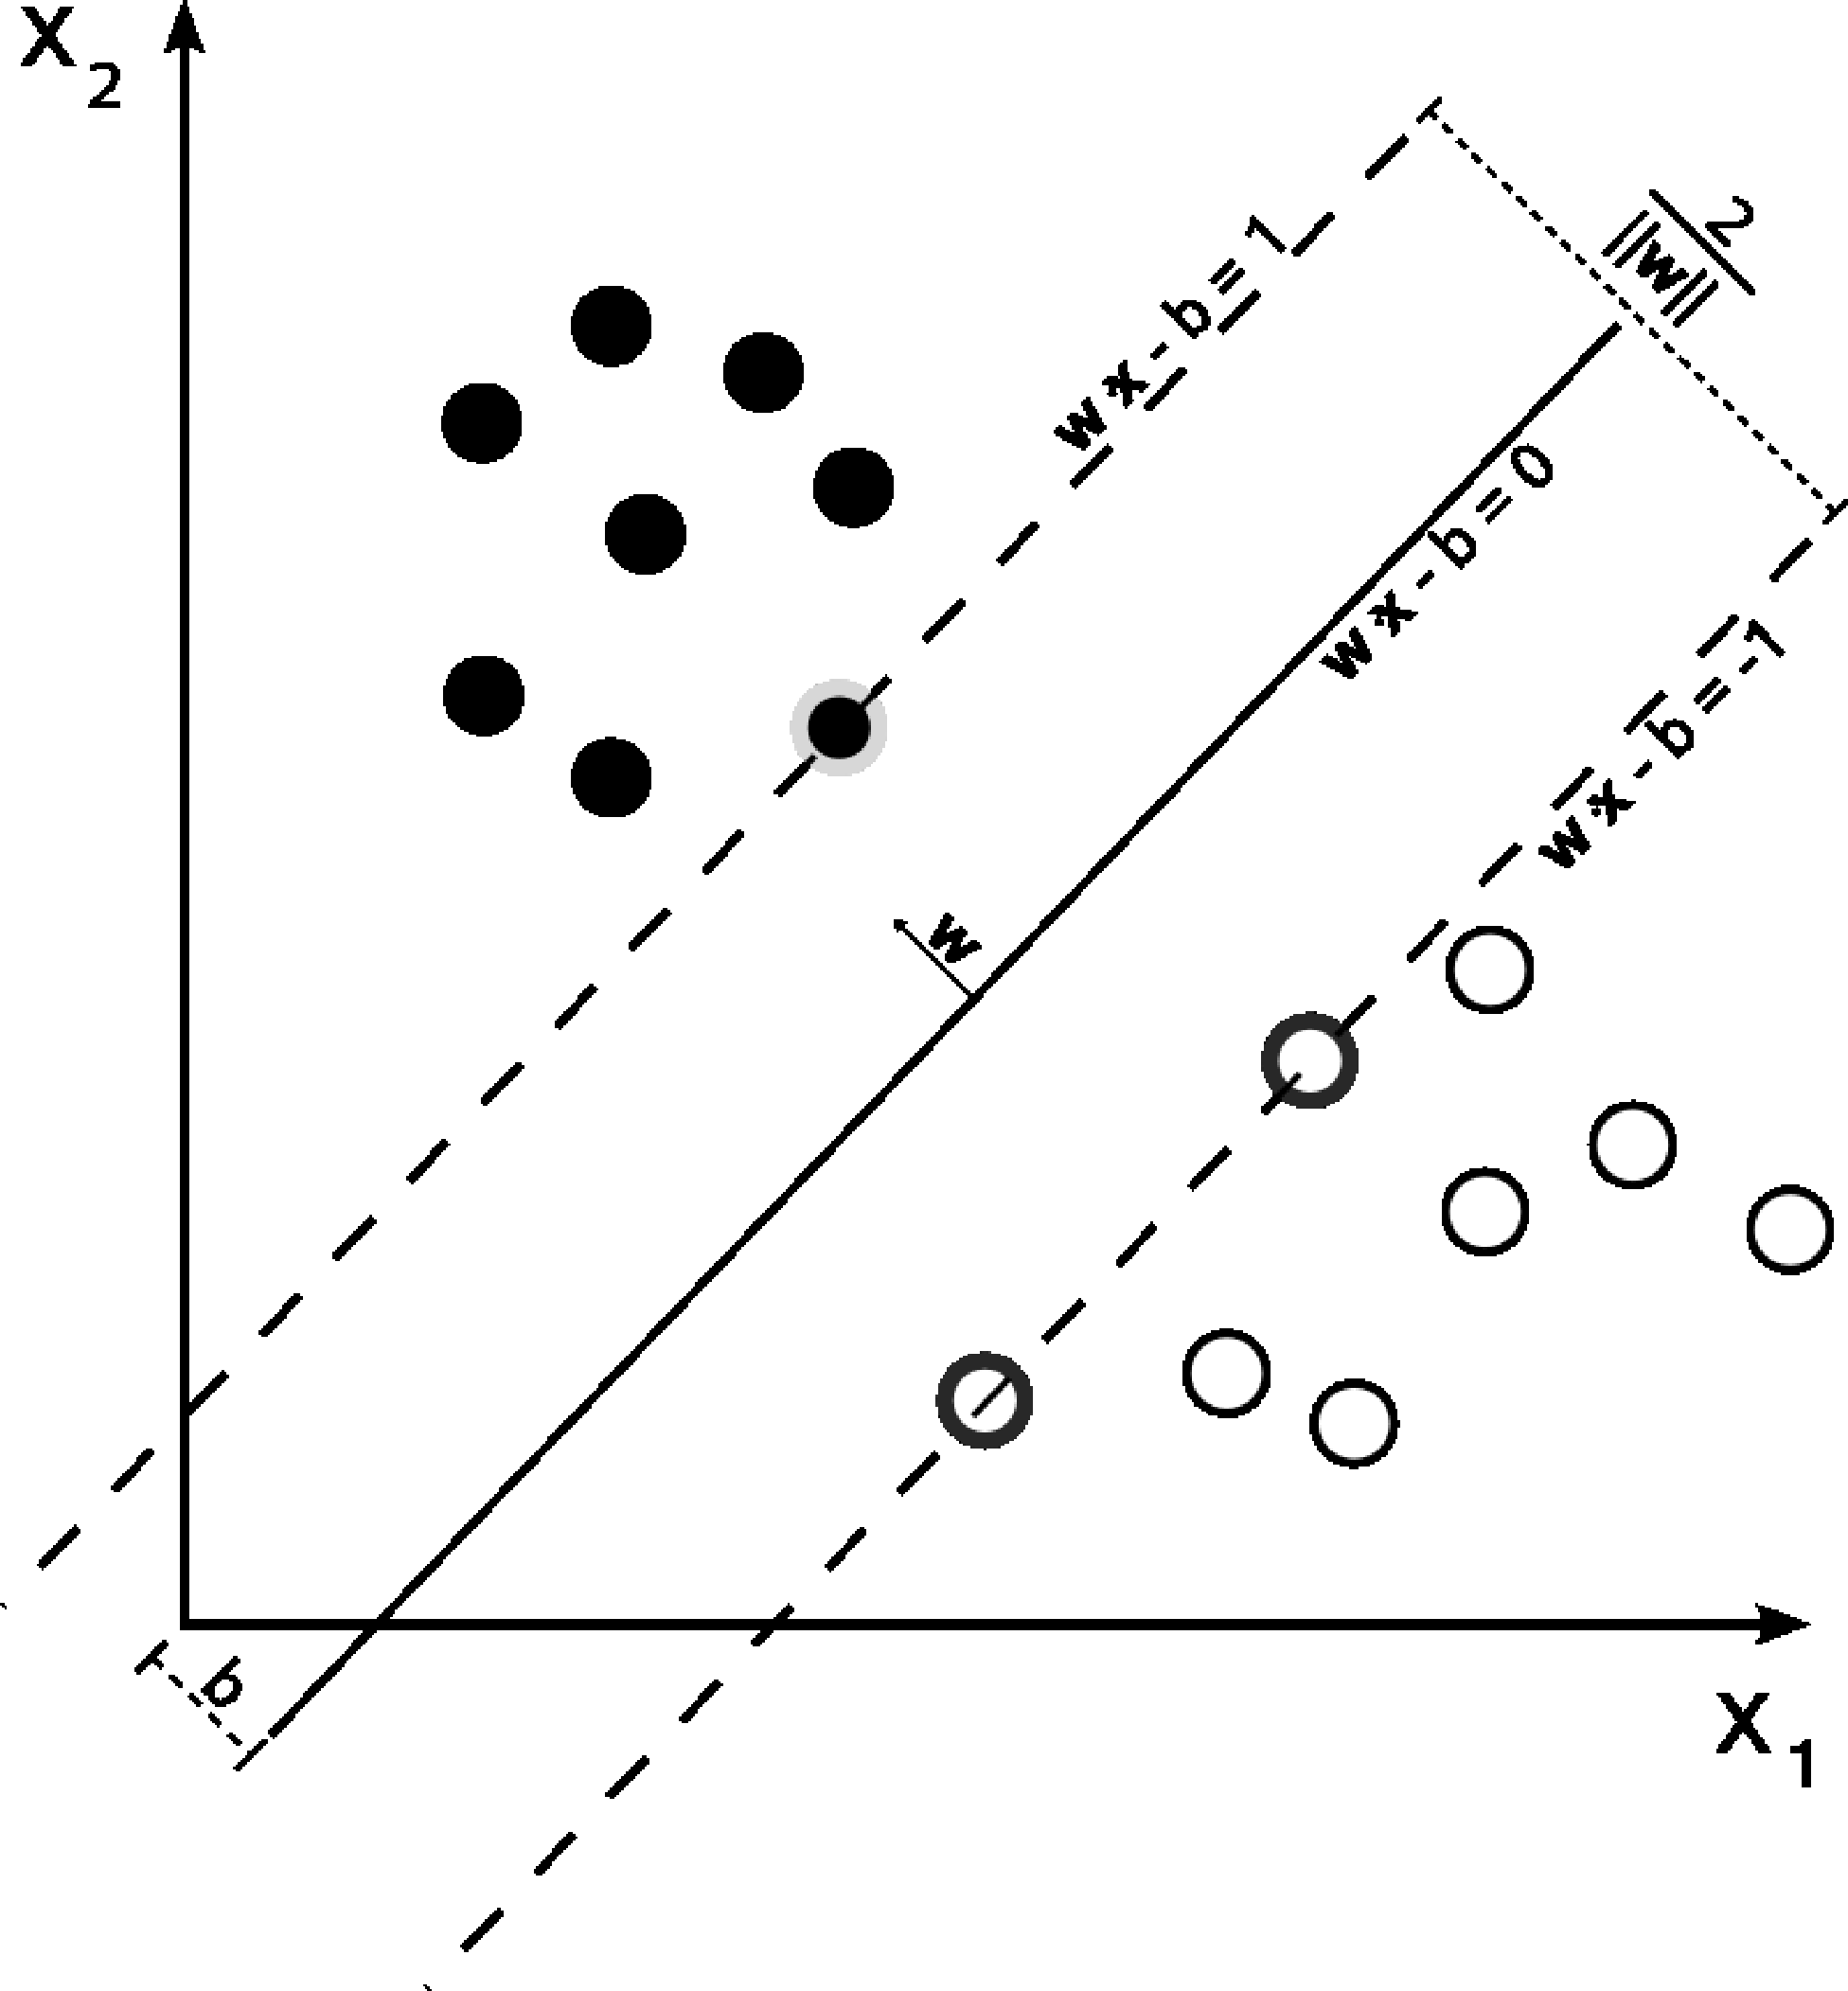
\includegraphics[width=0.8\textwidth]{Svm_max_sep_hyperplane_with_margin.png}
\caption{Intuitive explanation for independence of SVM from prior probabilities}
\label{Flo:SVM_balance}
\end{figure}


To get better results, we exclude the following attributes from the
dataset: {}``ID, location, n\_tags, maker''. Kernel of SVM is selected
to be RBF (radius basis function). Usually in real world applications,
data tends to scatter around circular clusters and hence this type
of kernel usually outperforms other kernels. An example of SVM with
this kernel is depicted in Figure \ref{Flo:Rbf}. Another major issue
is that all classifiers need the target to be nominal, hence we need
to change the favorite attribute from numerical to nominal. This
is simply done by using discrete filter in Weka with 10 bins. Histogram
after discretization is shown in Figure \ref{Flo:disc}. As expected,
classification results are really glamorous with SVM: 95.7\% of samples
are correctly classified. We note that 2/3 of data was selected as
training set and the rest was used for testing. We also tested our
technique with J48 tree, and with the same settings. This time we
got 85.9\% correct classification.

Now we get to our main purpose of this analysis, which is to study
the role of camera model in the classification result. We exclude
camera model from the attributes and use both SVM and J48 classifiers.

%
\begin{figure}
\centering
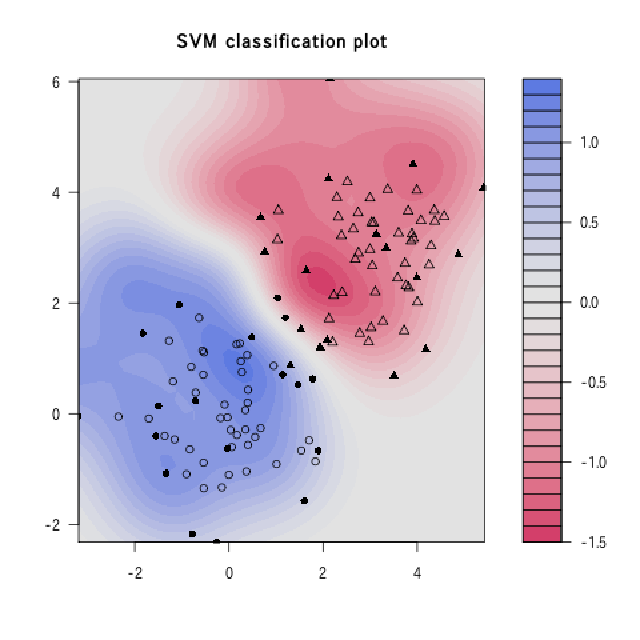
\includegraphics[width=0.8\textwidth]{svm_rbf.png}
\caption{An example of SVM with RBF kernel, which shows the characteristics
of this kernel.}
\label{Flo:Rbf}
\end{figure}


%
\begin{figure}
\centering
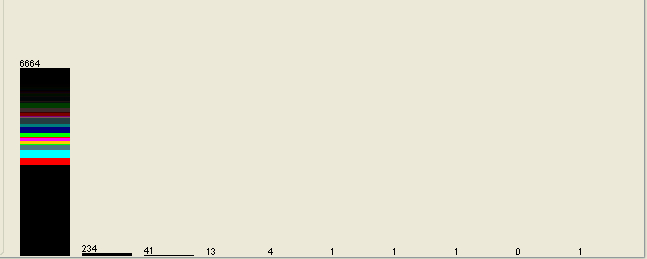
\includegraphics[width=0.8\textwidth]{hist_disc.png}
\caption{Histogram of favorite attribute after discretization}
\label{Flo:disc}
\end{figure}



\section{Discussion}

The Flickr API provides a wonderful opportunity to explore very interesting datasets. However, an important point to consider in order to get meaningful results is the sampling strategy. While the sampling strategy we used is reasonable, there are other ways to sample the data that should be explored.

It was not surprising that our data showed a long tail behavior, since this is typical for data originated on social networks. This fact leads us to think that it would be interesting to investigate some techniques specially tailored to this kind of distribution.

This work triggers some new interesting question that could be answering by mining Flickr, like for instance:
\begin{itemize}
\item Using geolocation information of the photos, can we identify a correlation between location and type of camera used? Producing, for examples, a statement like. ``people in the USA use mostly Canon cameras, while people in Europe use mostly Nikon''.
\item So far we ignored the users, but some patterns may arise by looking at this dimension. For instance we could try to answer questions like, ``are some users with a lot of popular photos?'', ``can we identify ``different classes'' of users?'', etc.
\item Can we found some semantic of the photos by looking at the data?
\end{itemize}

\bibliographystyle{plain}
\bibliography{report}
\end{document} 